\documentclass[11pt]{article}
\usepackage[margin=1in]{geometry}
\usepackage{graphicx}
\usepackage{booktabs}
\usepackage{amsmath}
\usepackage{amssymb}
\usepackage{float}
\usepackage[T1]{fontenc}
\usepackage{hyperref}

\title{Update (April 22): DBSCAN on 4 Phone Classes \\ with an MCMC-Sampled GMM Core Diagnostic}
\author{}
\date{}

\begin{document}
\maketitle
\thispagestyle{empty}

\section*{Summary}

Following the previous 5-class experiment, I narrowed the problem to 4 acoustically distinct phone classes --- \texttt{aa} (open back vowel), \texttt{n} (nasal), \texttt{sh} (voiceless postalveolar fricative), and \texttt{sil} (silence) --- so that a perfect algorithm should, in principle, find four physically separate density blobs in 12D MFCC space.

Two notebooks were run:
\begin{enumerate}
\item \texttt{dbscan\_4phone\_classes\_dim12.ipynb} --- standard DBSCAN on the raw standardized 12D MFCC frames. Best tuned run gave 4 clusters but with \textbf{64\%} of points labelled noise and one dominant cluster absorbing most of the signal (NMI $= 0.3088$, ARI $= 0.2293$).
\item \texttt{dbscan\_4phone\_mcmc\_gmm\_dim12.ipynb} --- fit a 4-component GMM, then Metropolis--Hastings sample from each component restricted to its high-density \emph{core} (Mahalanobis distance $\leq 1.5\sigma$). DBSCAN on this synthetic core dataset achieves \textbf{NMI $= 0.9990$, ARI $= 0.9995$} with 99.96\% coverage --- near-perfect recovery of all 4 classes.
\end{enumerate}

The sharp gap between the two runs isolates the cause: DBSCAN's failure on raw MFCC frames is driven by overlapping tails between phone distributions, not by the DBSCAN algorithm itself. Transferring the core-tuned $(\varepsilon, \text{min\_samples})$ back to the real frames still fails (NMI $= 0.23$, 85\% noise), which means the fix has to happen upstream of clustering --- either in feature design or by core-posterior filtering of frames before clustering.

\section*{Setup}

\paragraph{Data.} \texttt{train\_dim12.json}, 4620 TIMIT utterances, 12-dim MFCC per frame. Frame-level labels expanded from \texttt{phn\_transcript}.

\paragraph{Class frame counts (full dataset).} Silence dominates:
\begin{table}[H]
\centering
\begin{tabular}{lr}
\toprule
Phoneme & Frame count \\
\midrule
\texttt{sil} & 367{,}150 \\
\texttt{aa}  &  73{,}885 \\
\texttt{n}   &  46{,}996 \\
\texttt{sh}  &  27{,}046 \\
\midrule
Total        & 515{,}077 \\
\bottomrule
\end{tabular}
\end{table}

\paragraph{Stratified subset.} 3{,}000 frames per class (12{,}000 total) are sampled uniformly at random without replacement, then standardized with \texttt{StandardScaler}. Stratification is required because DBSCAN's global density estimate would otherwise be set by \texttt{sil} alone.

\section*{Notebook 1: DBSCAN on Raw MFCC Frames}

\subsection*{Methodology}

\begin{itemize}
\item \textbf{Preprocessing:} \texttt{StandardScaler} on the 12D MFCCs (required because $c_0$ log-energy has an order-of-magnitude larger range than $c_1$--$c_{11}$, and DBSCAN uses plain Euclidean distance).
\item \textbf{Hyperparameter guidance:} $k$-distance curves at $k \in \{8, 12, 20\}$ (distance to the $k$-th nearest neighbor, sorted). The quantile table below drives the $\varepsilon$ grid. Elbows sit around 1.7--2.3 in standardized distance units.
\item \textbf{Sweep:} $\varepsilon \in [1.0, 2.0]$ (step 0.1), $\text{min\_samples} \in \{6, 8, 10, 12, 15, 20\}$. Sorted first by $|\text{clusters} - 4|$, then by NMI, then by noise fraction.
\end{itemize}

\begin{table}[H]
\centering
\caption{$k$-distance quantiles on the 12{,}000-point standardized subset.}
\begin{tabular}{lrrrrr}
\toprule
$k$ & $q_{50}$ & $q_{75}$ & $q_{90}$ & $q_{95}$ & $q_{99}$ \\
\midrule
 8 & 1.6765 & 1.9636 & 2.2508 & 2.4404 & 2.8311 \\
12 & 1.7713 & 2.0680 & 2.3711 & 2.5688 & 2.9652 \\
20 & 1.8898 & 2.2072 & 2.5202 & 2.7245 & 3.1419 \\
\bottomrule
\end{tabular}
\end{table}

\subsection*{Results}

Best 4-cluster configuration: $\varepsilon = 1.4$, $\text{min\_samples} = 12$.

\begin{table}[H]
\centering
\caption{Best DBSCAN runs on raw 4-class frames (top of ranked sweep).}
\begin{tabular}{rrrrrrr}
\toprule
min\_samples & $\varepsilon$ & clusters & noise frac. & NMI & ARI & Homogeneity \\
\midrule
12 & 1.4 & 4 & 0.6432 & 0.3088 & 0.2293 & 0.2292 \\
10 & 1.4 & 4 & 0.6288 & 0.3055 & 0.2332 & 0.2283 \\
10 & 1.8 & 4 & 0.2177 & 0.1053 & 0.0535 & 0.0732 \\
 8 & 1.9 & 4 & 0.1262 & 0.0610 & 0.0165 & 0.0391 \\
\bottomrule
\end{tabular}
\end{table}

Only the first two configurations have meaningful structure; the low-noise runs at larger $\varepsilon$ collapse everything into one cluster (near-zero NMI). Selected run at $\varepsilon = 1.4$, $\text{min\_samples} = 12$:

\begin{itemize}
\item Clusters found: 4
\item Noise fraction: 0.6432 (coverage 0.3568)
\item AMI $= 0.3084$, NMI $= 0.3088$, ARI $= 0.2293$, Homogeneity $= 0.2292$, Completeness $= 0.4730$
\end{itemize}

\begin{table}[H]
\centering
\caption{Cluster composition. Cluster 0 holds 99\% of clustered points; clusters 1--3 are micro-clusters.}
\begin{tabular}{rrlrr}
\toprule
Cluster & Size & Majority phone & Purity & \# unique phones \\
\midrule
0 & 4246 & \texttt{sh} & 0.5810 & 4 \\
1 &    6 & \texttt{n}  & 0.6667 & 2 \\
2 &   20 & \texttt{n}  & 0.9500 & 2 \\
3 &   10 & \texttt{n}  & 1.0000 & 1 \\
\bottomrule
\end{tabular}
\end{table}

\begin{table}[H]
\centering
\caption{Crosstab, true phone $\times$ DBSCAN cluster (column $-1$ = noise).}
\begin{tabular}{lrrrrr}
\toprule
true $\backslash$ cluster & $-1$ & 0 & 1 & 2 & 3 \\
\midrule
\texttt{aa}  & 2997 &    3 &  0 &  0 &  0 \\
\texttt{n}   & 2841 &  126 &  4 & 19 & 10 \\
\texttt{sh}  &  533 & 2467 &  0 &  0 &  0 \\
\texttt{sil} & 1347 & 1650 &  2 &  1 &  0 \\
\bottomrule
\end{tabular}
\end{table}

Reading the crosstab: cluster 0 is essentially a \texttt{sh}+\texttt{sil} blob with heavy \texttt{n} and \texttt{aa} contamination; \texttt{aa} (2997) and \texttt{n} (2841) are almost entirely noise. DBSCAN technically finds 4 clusters but only one is non-trivial, and that one is \emph{mixed}.

\subsection*{Figures}

\begin{figure}[H]
\centering
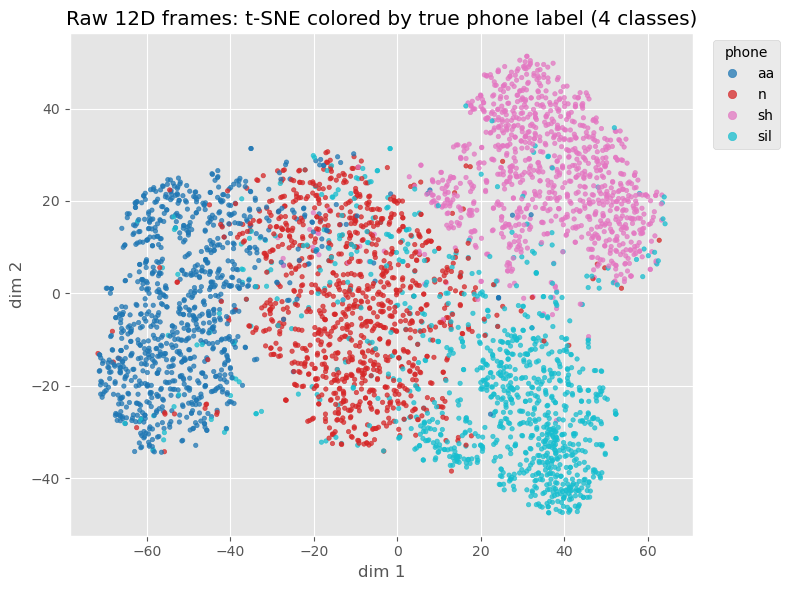
\includegraphics[width=0.75\textwidth]{assets/nb1_truth_tsne.png}
\caption{Ground-truth t-SNE of 4{,}000 raw standardized frames (12D $\to$ 2D), colored by true phone. \texttt{sh} forms a distinct cloud; \texttt{aa}, \texttt{n}, \texttt{sil} overlap heavily along their boundaries.}
\end{figure}

\begin{figure}[H]
\centering
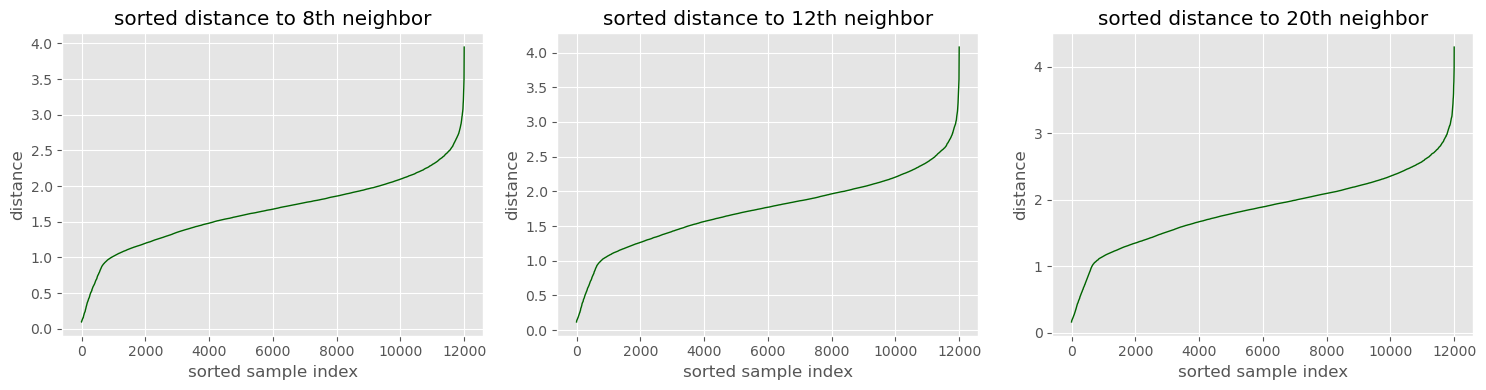
\includegraphics[width=\textwidth]{assets/nb1_kdistance.png}
\caption{$k$-distance curves at $k = 8, 12, 20$. The gentle rise with no sharp elbow explains why DBSCAN struggles: there is no clear density transition at any single $\varepsilon$.}
\end{figure}

\begin{figure}[H]
\centering
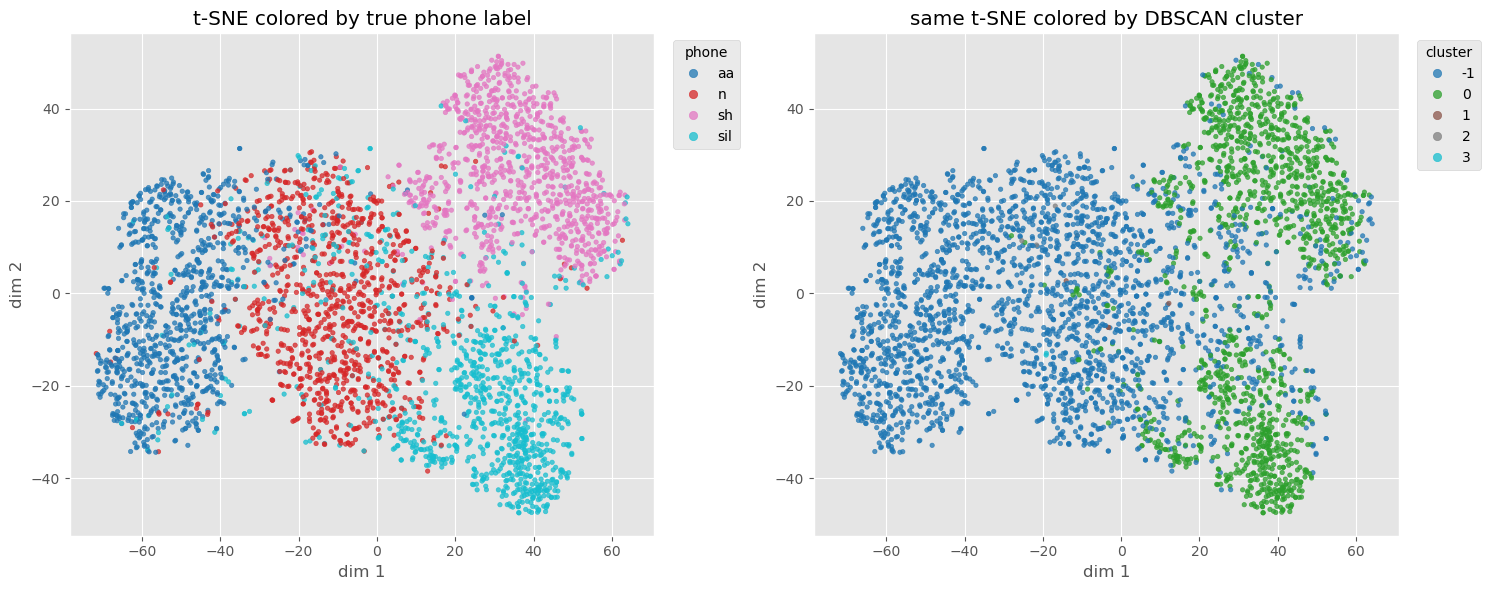
\includegraphics[width=\textwidth]{assets/nb1_truth_vs_dbscan_tsne.png}
\caption{Same 2D embedding colored by true phone (left) vs DBSCAN cluster (right). The right panel shows one dominant cluster and a majority-noise background --- the density structure is not four discrete cores.}
\end{figure}

\section*{Notebook 2: MCMC-Sampled GMM Cores}

\subsection*{Motivation}

DBSCAN defines clusters as dense regions separated by sparser ones. On the raw 4-class MFCC frames, there is no density gap between classes --- the tails of \texttt{aa}, \texttt{n}, and \texttt{sil} overlap. If we strip those tails and keep only high-density cores, the density gap should reappear and DBSCAN should work. This notebook is a diagnostic to test exactly that claim.

\subsection*{Methodology}

\paragraph{Step 1 --- GMM.} Fit a 4-component GMM on the stratified standardized subset with \texttt{covariance\_type="full"}. To lock each component to a phone rather than let EM reshuffle them, \texttt{means\_init} is set to the per-phone sample means and \texttt{weights\_init} to the per-phone frequencies. The final component-to-phone mapping (after reordering by nearest mean) is $\{0:\texttt{aa},\ 1:\texttt{n},\ 2:\texttt{sh},\ 3:\texttt{sil}\}$ with weights $[0.256, 0.417, 0.247, 0.081]$.

\paragraph{Step 2 --- Metropolis--Hastings core sampling.} For each component $k$ with fitted $(\mu_k, \Sigma_k)$, sample from the target
\[
\pi_k(x) \;\propto\; \mathcal{N}(x;\mu_k,\Sigma_k) \,\cdot\, \mathbf{1}\!\left[d_M(x,\mu_k)\le\tau\right],
\]
where $d_M(x,\mu_k) = \sqrt{(x-\mu_k)^\top \Sigma_k^{-1} (x-\mu_k)}$ is the Mahalanobis distance and $\tau = 1.5$. The indicator zeros out the tails, and Metropolis--Hastings with a symmetric Gaussian random-walk proposal $\mathcal{N}(0, s^2 \Sigma_k)$, $s = 0.25$, draws samples from the restricted target.

Burn-in $= 500$, thinning $= 3$, 2{,}000 kept samples per component (8{,}000 total). The scale $s = 0.25$ was tuned empirically to give $\approx 30\%$ acceptance, close to the optimal Metropolis regime in high dimension. Note that $\tau = 1.5\sigma$ in 12D corresponds to only $P(\chi^2_{12} \le 1.5^2) \approx 0.108\%$ of the Gaussian mass --- by design, this is a tight core.

\paragraph{Observed acceptance rates:}
\begin{center}
\begin{tabular}{lc}
\toprule
Component & MH acceptance rate \\
\midrule
\texttt{aa}  & 0.308 \\
\texttt{n}   & 0.313 \\
\texttt{sh}  & 0.309 \\
\texttt{sil} & 0.313 \\
\bottomrule
\end{tabular}
\end{center}

\paragraph{Step 3 --- DBSCAN sweep on the synthetic cores.} Grid over $\varepsilon \in [0.4, 2.0]$ (step 0.1) and $\text{min\_samples} \in \{5, 8, 10, 15, 20\}$. Same ranking rule.

\subsection*{Sanity Check Before Clustering}

\begin{figure}[H]
\centering
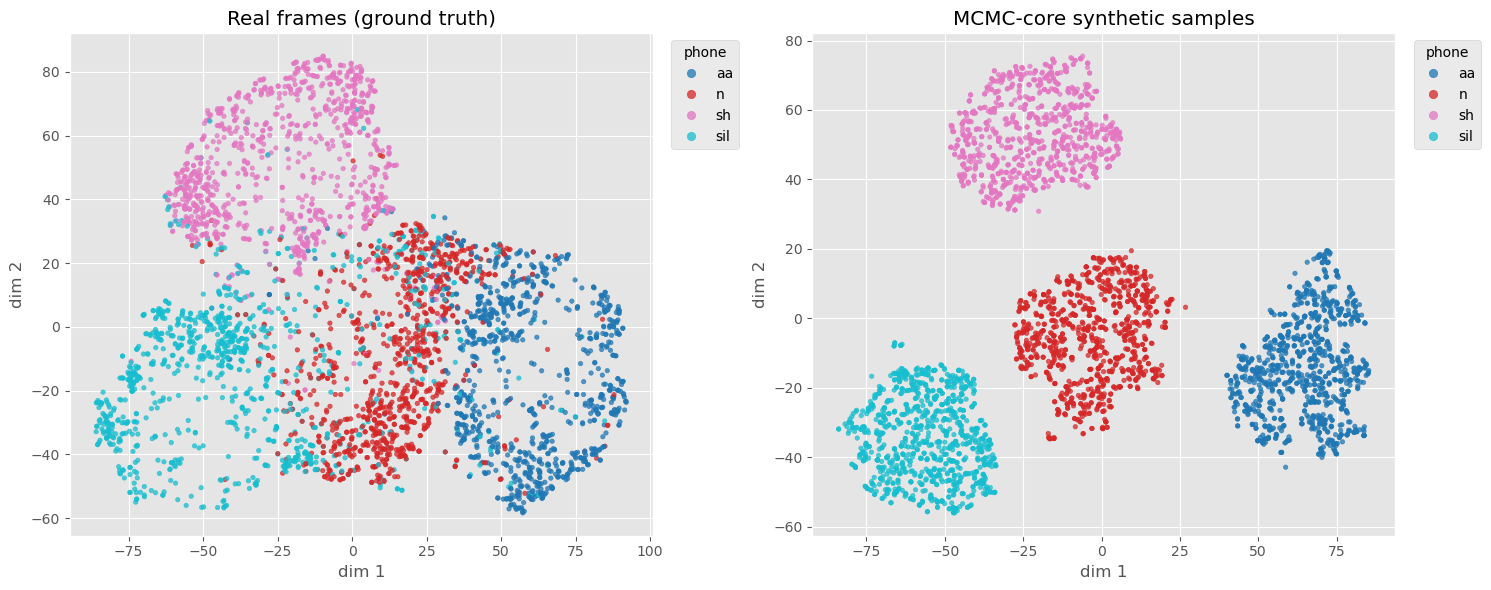
\includegraphics[width=\textwidth]{assets/nb2_real_vs_core_tsne.png}
\caption{t-SNE of the real standardized frames (left) and the MCMC-sampled GMM cores (right), computed \emph{jointly} so the 2D geometry is shared. The right panel shows four tight, well-separated blobs, confirming that the MCMC sampler is drawing from the high-density interior of each component. This is the geometry DBSCAN needs.}
\end{figure}

\begin{figure}[H]
\centering
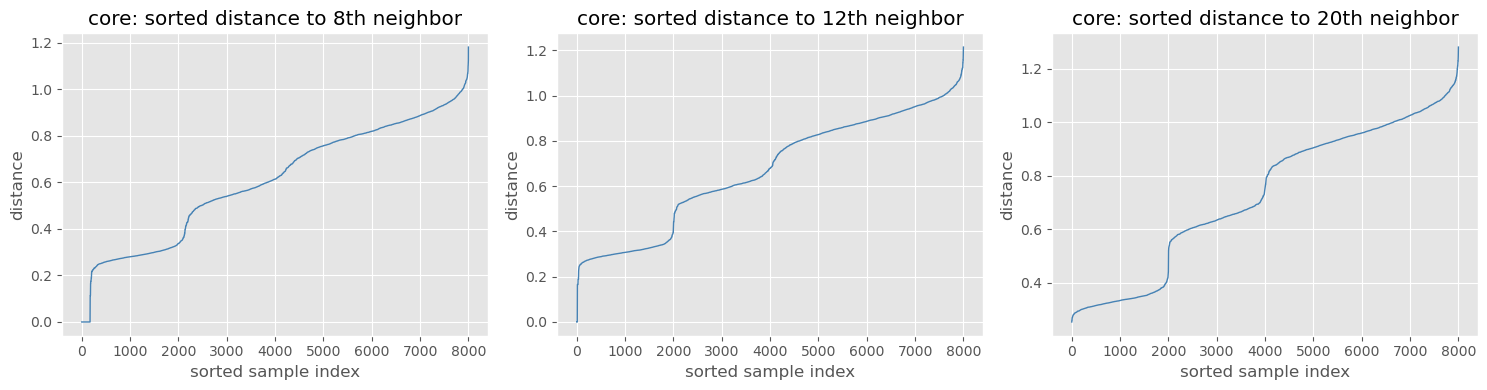
\includegraphics[width=\textwidth]{assets/nb2_core_kdistance.png}
\caption{$k$-distance curves on the core dataset. Typical distances are $\approx 0.7$--$1.0$, i.e. roughly half of the raw-frame scale (1.7--2.3). The elbow is also sharper, suggesting a well-defined density gap.}
\end{figure}

\subsection*{Results}

Best run: $\varepsilon = 1.0$, $\text{min\_samples} = 5$.

\begin{table}[H]
\centering
\caption{Best DBSCAN runs on MCMC-sampled cores (top of ranked sweep).}
\begin{tabular}{rrrrrrr}
\toprule
min\_samples & $\varepsilon$ & clusters & noise frac. & NMI & ARI & Homogeneity \\
\midrule
 5 & 1.0 & 4 & 0.0004 & 0.9990 & 0.9995 & 1.0000 \\
 8 & 1.0 & 4 & 0.0005 & 0.9987 & 0.9993 & 1.0000 \\
10 & 1.0 & 4 & 0.0008 & 0.9982 & 0.9990 & 1.0000 \\
15 & 1.0 & 4 & 0.0034 & 0.9936 & 0.9955 & 1.0000 \\
20 & 1.0 & 4 & 0.0100 & 0.9846 & 0.9871 & 0.9995 \\
\bottomrule
\end{tabular}
\end{table}

Selected run ($\varepsilon = 1.0$, $\text{min\_samples} = 5$):

\begin{itemize}
\item Clusters found: 4
\item Noise fraction: 0.0004 (coverage 0.9996)
\item AMI $= 0.9990$, NMI $= 0.9990$, ARI $= 0.9995$
\end{itemize}

\begin{table}[H]
\centering
\caption{Crosstab on the core dataset. Only 3 \texttt{aa} points fall in a spurious micro-cluster; the remaining 7{,}997 are clustered perfectly by true class. Column $-1$ is the noise column; each of columns 1--4 aligns one-to-one with a phone.}
\begin{tabular}{lrrrrr}
\toprule
true $\backslash$ cluster & $-1$ & 1 & 2 & 3 & 4 \\
\midrule
\texttt{aa}  &  3 & 1997 &    0 &    0 &    0 \\
\texttt{n}   &  0 &    0 & 2000 &    0 &    0 \\
\texttt{sh}  &  0 &    0 &    0 & 2000 &    0 \\
\texttt{sil} &  0 &    0 &    0 &    0 & 2000 \\
\bottomrule
\end{tabular}
\end{table}

\begin{figure}[H]
\centering
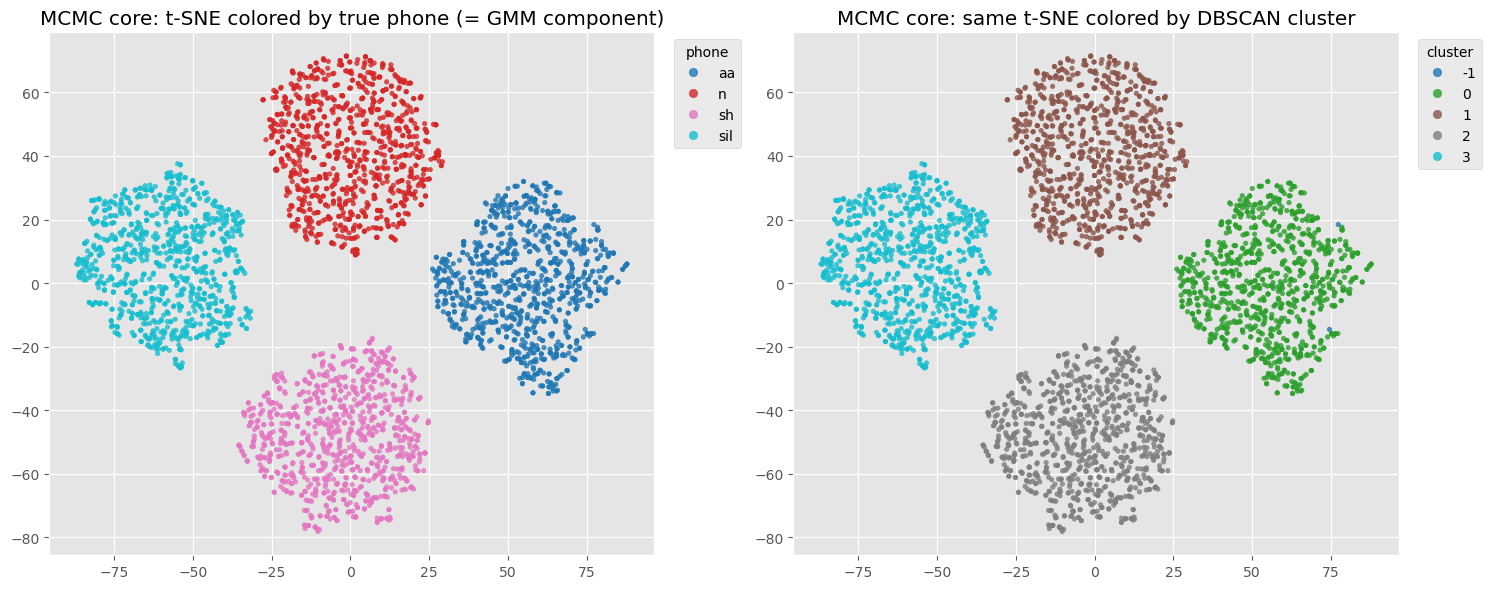
\includegraphics[width=\textwidth]{assets/nb2_core_truth_vs_dbscan_tsne.png}
\caption{MCMC core dataset t-SNE: truth (left) vs DBSCAN (right). The two panels are visually identical --- DBSCAN recovers the component structure almost perfectly when the tails are absent.}
\end{figure}

\subsection*{Transfer Back to Real Frames}

A natural follow-up: does the $(\varepsilon, \text{min\_samples})$ chosen on the cores work when applied directly to the real standardized frames? No.

\begin{itemize}
\item Configuration transferred: $\varepsilon = 1.0$, $\text{min\_samples} = 5$
\item Clusters found on real frames: 11
\item Noise fraction: 0.8484
\item NMI $= 0.2302$, ARI $= 0.0456$
\end{itemize}

The real frames have larger typical neighbor distances than the cores (the core cluster radius is about half that of the raw data), so $\varepsilon = 1.0$ is simply too small on the real data --- 85\% of points become noise, and the surviving 15\% fragment into 11 micro-clusters. This is the expected failure mode and confirms the interpretation.

\section*{Interpretation and Takeaway}

\begin{table}[H]
\centering
\caption{Side-by-side summary of the two notebooks.}
\begin{tabular}{lcccc}
\toprule
Setup & Clusters & Coverage & NMI & ARI \\
\midrule
Raw frames (best DBSCAN) & 4 & 0.3568 & 0.3088 & 0.2293 \\
MCMC cores (best DBSCAN) & 4 & 0.9996 & 0.9990 & 0.9995 \\
Core-tuned config, transferred to real frames & 11 & 0.1516 & 0.2302 & 0.0456 \\
\bottomrule
\end{tabular}
\end{table}

\paragraph{What this rules out.} DBSCAN is not the bottleneck. The same algorithm with the same sweep protocol on the same feature dimensionality achieves NMI $\approx 1$ once overlapping tails are removed. A further shrinkage of the class set below 4 is therefore not expected to help much --- the remaining mass overlap between \texttt{aa}, \texttt{n}, \texttt{sil} in 12D MFCC space is the real obstacle.

\paragraph{What the experiments point to.} Two directions are consistent with these results:
\begin{enumerate}
\item Replace raw MFCCs with a feature where the \emph{tails} of each phone class are narrower --- e.g. context-windowed MFCCs (already explored in \texttt{dbscan\_variants\_5phone.ipynb}), or learned bottleneck features from a phone classifier.
\item Keep raw MFCCs but combine clustering with a \emph{core filter}: fit a GMM, retain only frames whose maximum posterior exceeds a threshold, run DBSCAN on the surviving frames. The transfer experiment above already shows this is mathematically similar to what the core notebook does; the practical difference is that the filter operates on \emph{real} data, so the evaluation has to be done against a held-out set.
\end{enumerate}

Compared to the previous 5-class run (best NMI $\approx 0.11$ with \texttt{s}, \texttt{ih}, \texttt{aa}, \texttt{iy}, \texttt{ae}), the 4-class raw-frame run is slightly better (NMI $\approx 0.31$) purely because \texttt{sh} and \texttt{sil} are spectrally distinctive. But the ceiling is still well below the near-1.0 that becomes available once tails are stripped, and that gap is the useful signal from this experiment.

\end{document}
